\documentclass{scrartcl}
\usepackage[ngerman]{babel}%[english]
\usepackage{graphicx}
\usepackage{amsmath}
\usepackage{amssymb}
\usepackage{amsfonts}
%\usepackage{booktabs}
\parindent0pt %keineinrücken
\usepackage[utf8]{inputenc}
\usepackage{placeins}
\usepackage{footnote}
\usepackage{capt-of}
\usepackage{listings}% TXT Dateien in LaTeX einbinden
\usepackage{comment} % über Zeilen hinweg Kommentare schreiben
\usepackage{fancyhdr}
\usepackage{geometry}
\usepackage{hyperref}
\usepackage{fancyvrb}% 2. Möglichkeit TXT Dateien in LaTeX einbinden
\hypersetup{pdftex=true, colorlinks=true, breaklinks=true, linkcolor=blue, menucolor=blue, pagecolor=blue, urlcolor=blue}
\usepackage{nicefrac}
\geometry{a4paper, bottom=2cm}%, portrait,left=1cm, right=1cm, top=2cm
\begin{document}
\lstset{language=c++,breaklines=true,numbers=left,frame=single,
extendedchars=true,inputencoding=utf8}
\lstset{literate=%
{Ö}{{\"O}}1 
{Ä}{{\"A}}1 
{Ü}{{\"U}}1 
{ß}{{\ss}}2 
{ü}{{\"u}}1 
{ä}{{\"a}}1 
{ö}{{\"o}}1
}
\pagestyle{fancy}
\lhead{Christian Gößl 762627\\ BaPh 6}
\rhead{\today}
\part*{Programm zur Erstellung von Periodogrammen}
\section{Einleitung}
Dieses Programm passiert auf den Ausführungen aus den Paper von Horne \& Baliunas (1986) \footnote{The Astrophysical Journal, 302:757-763, 1986 March 15 Horne \& Baliunas http://adsabs.harvard.edu/abs/1986ApJ...302..757H}, worin eine Methode zur Berechnung von Periodogrammen vorgestellt wird. Diese Periodogramme sind das Ergebnis einer Fouriertransformation mit den Erweiterungen aus dem Paper. Das Programm ist in der Programmiersprache C++ geschrieben und kann zur Auswertung von Zeitreihen benutzt werden. Der vollständige Quellcode kann im Appendix eingesehen werden.

\section{Funktionen des Programms}

Es kann eine Zeitreihe in dieser Form (t,x,$\sigma$) eingelesen werden, daraus wird ein Periodogramm und im aktuellen Verzeichnis die Ergebnisdaten im Format ($\omega$ , Amplitude) in einer Datei mit dem Namen \textit{Fourier-} am Anfang erstellt. Die Zeitreihe wird zur weiteren Verarbeitung in 2 Felder gespeichert. Beim Start des Programms wird der Nutzer aufgefordert den Namen der zu untersuchende Datei einzugeben, gefolgt mit der Eingabe der größtmöglichen gewollten Frequenz $\omega$. Dies wird durch die Funktion initial bereitgestellt. 

\lstinputlisting[firstnumber=40,firstline=40,lastline=49]{Hausarbeit.cpp}

Diese und weitere Funktion werden in der Prozedur \textit{main} gestartet.

\lstinputlisting[firstnumber=22,firstline=22,lastline=38]{Hausarbeit.cpp}

Zu Testzwecken kann der Name \textit{TestDaten.dat} mit $ \omega = 10 $ eingeben werden, der Name der Ausgabedatei lautet dann \textit{Fourier-TestDaten.dat}. Die TestDaten werden in der Funktion \textit{BuildSignal} erzeugt, dabei wird zu einer Cosinus Funktion ein Gaußsches Rauschen aufaddiert. 

\lstinputlisting[firstnumber=51,firstline=51,lastline=72]{Hausarbeit.cpp}

Den Median der Zeitreihe wird in der Funktion \textit{median} berechnet, wobei ein Sortieralgorithmus (Minimumsuche) verwendet wird. 

\lstinputlisting[firstnumber=160,firstline=160,lastline=200]{Hausarbeit.cpp}

Der Median wird dann in der Funktion \textit{FourierTrafo} verwendet. Dort werden die Formeln zur Berechnung der Fouriertransformation aus dem Paper von Horne \& Baliunas (1986) verwendet. Aus einer Zeitreihe $ X(t_j) $ mit $ i = 1, ... , N_0 $ wird ein Periodogramm erzeugt mit der folgenden Funktion $ P_X(\omega) $. Zu beachten ist das hier zusätzlich der Median $ X_{med} $ bei der Zeitreihe vorher abgezogen wird.

\begin{align*}
	P_X (\omega) & = \frac{1}{2}\left( \frac{\left[ \sum_{j=1}^{N_0}(X(t_j) - X_{med})cos(\omega (t_j - \tau) \right]^2 }{\sum_{j=1}^{N_0}(X(t_j) - X_{med})cos^2(\omega (t_j - \tau)} + \frac{\left[ \sum_{j=1}^{N_0}(X(t_j) - X_{med})sin(\omega (t_j - \tau) \right]^2 }{\sum_{j=1}^{N_0}(X(t_j) - X_{med})sin^2(\omega (t_j - \tau)} \right) \\
	& tan(2\omega \tau)  =\nicefrac{\left(\sum_{j=1}^{N_0}sin(2\omega t_j ) \right)}{\left(\sum_{j=1}^{N_0}cos(2\omega t_j ) \right)} 
\end{align*}

Diese Funktion muss noch normiert werden mit der absoluten Varianz.

\begin{align*}
	\sigma^2 & = \sum_{j=1}^{N_0}(X(t_j)- X_{med})^2 \\
 	P_N(\omega ) & = \nicefrac{P_X(\omega ) }{\sigma ^2} 
\end{align*}

\lstinputlisting[firstnumber=101,firstline=101,lastline=144]{Hausarbeit.cpp}

Zusätzlich wird die Frequenz $ \omega _0 $ des stärksten Signals gesucht und in die Ausgabedatei geschrieben.

\lstinputlisting[firstnumber=134,firstline=134,lastline=143]{Hausarbeit.cpp}

\section{Anwendung des Programms}

Zur Anwendung werden die folgenden Zeitreihen verwendet \textit{lmc-cepheid.dat}, \textit{x-ray.dat} und \textit{doubleP.dat}. Die sich ergebenden Periodogramme wurden mittels Gnuplot ausgewertet (Siehe Abb. \ref{pic:periodo}). Der Gnuplot Code zur Erzeugung der Diagramme befindet sich im Appendix.

\begin{figure}[htp!]
\begin{center}
		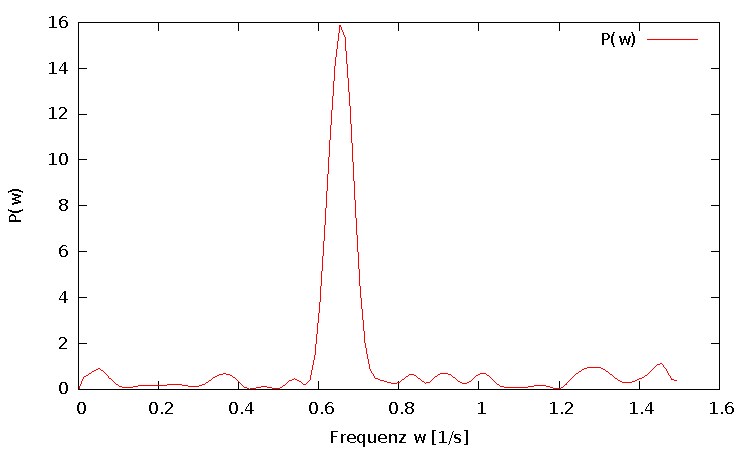
\includegraphics[width=0.8\textwidth]{plot-lmc-cepheid.pdf}
		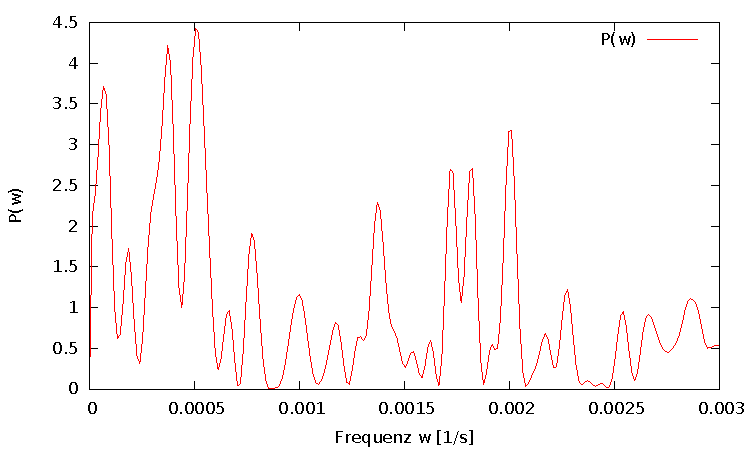
\includegraphics[width=0.8\textwidth]{plot-x-ray.pdf}
		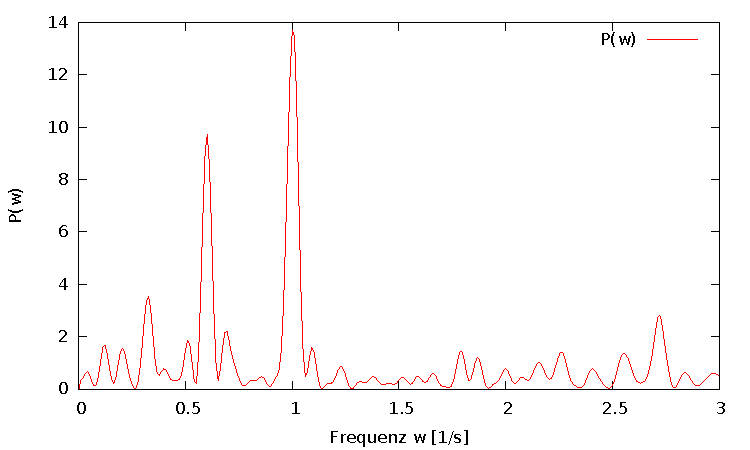
\includegraphics[width=0.8\textwidth]{plot-doubleP.pdf}
	\caption{Periodogramme der Datensätze v.o.n.u \textit{lmc-cepheid.dat}, \textit{x-ray.dat} und \textit{doubleP.dat}}
	\label{pic:periodo}
\end{center}
\end{figure}
\newpage
\section{Appendix}
\subsection{gesamter Quellcode}
\lstinputlisting{Hausarbeit.cpp}
\subsection{Gnuplot Code}
\lstinputlisting{plot.plt}
\end{document}